% =============================================================================
% cover-template.tex – Universelle Vorlage für techdoc.cls Cover
% =============================================================================
% Kompilieren: xelatex cover-template.tex
% Erzeugt: cover-template.pdf (umbenennen für \coverimage in main.tex)
%
% ANPASSUNG:
% 1. Titel und Untertitel ändern (Zeile ~75)
% 2. Inhalt im CONTENT-Bereich anpassen (ab Zeile ~85)
% 3. Datei umbenennen: cover-[thema].tex
% =============================================================================
\documentclass[tikz,border=0pt]{standalone}

% -----------------------------------------------------------------------------
% SCHRIFTEN (identisch mit techdoc.cls)
% -----------------------------------------------------------------------------
\usepackage{fontspec}
\defaultfontfeatures{Ligatures=TeX}

\setmainfont{TeX Gyre Pagella}
\setsansfont{TeX Gyre Heros}
\setmonofont[Scale=0.85]{TeX Gyre Cursor}

% -----------------------------------------------------------------------------
% FARBEN (identisch mit techdoc.cls)
% -----------------------------------------------------------------------------
\usepackage{xcolor}

% Primärfarben
\definecolor{ArduinoTeal}{HTML}{00979D}
\definecolor{ArduinoDark}{HTML}{005C5F}
\definecolor{RaspberryRed}{HTML}{C51A4A}

% Statusfarben
\definecolor{SuccessGreen}{HTML}{75A928}
\definecolor{WarningOrange}{HTML}{D97706}

% Neutrale Farben
\definecolor{MutedText}{HTML}{4A5568}
\definecolor{CodeBg}{HTML}{F8FAFC}
\definecolor{CodeFrame}{HTML}{C8D2DC}

% -----------------------------------------------------------------------------
% TIKZ-BIBLIOTHEKEN
% -----------------------------------------------------------------------------
\usetikzlibrary{shapes, arrows.meta, positioning, calc, decorations.pathreplacing}

% -----------------------------------------------------------------------------
% WIEDERVERWENDBARE STILE
% -----------------------------------------------------------------------------
\begin{document}
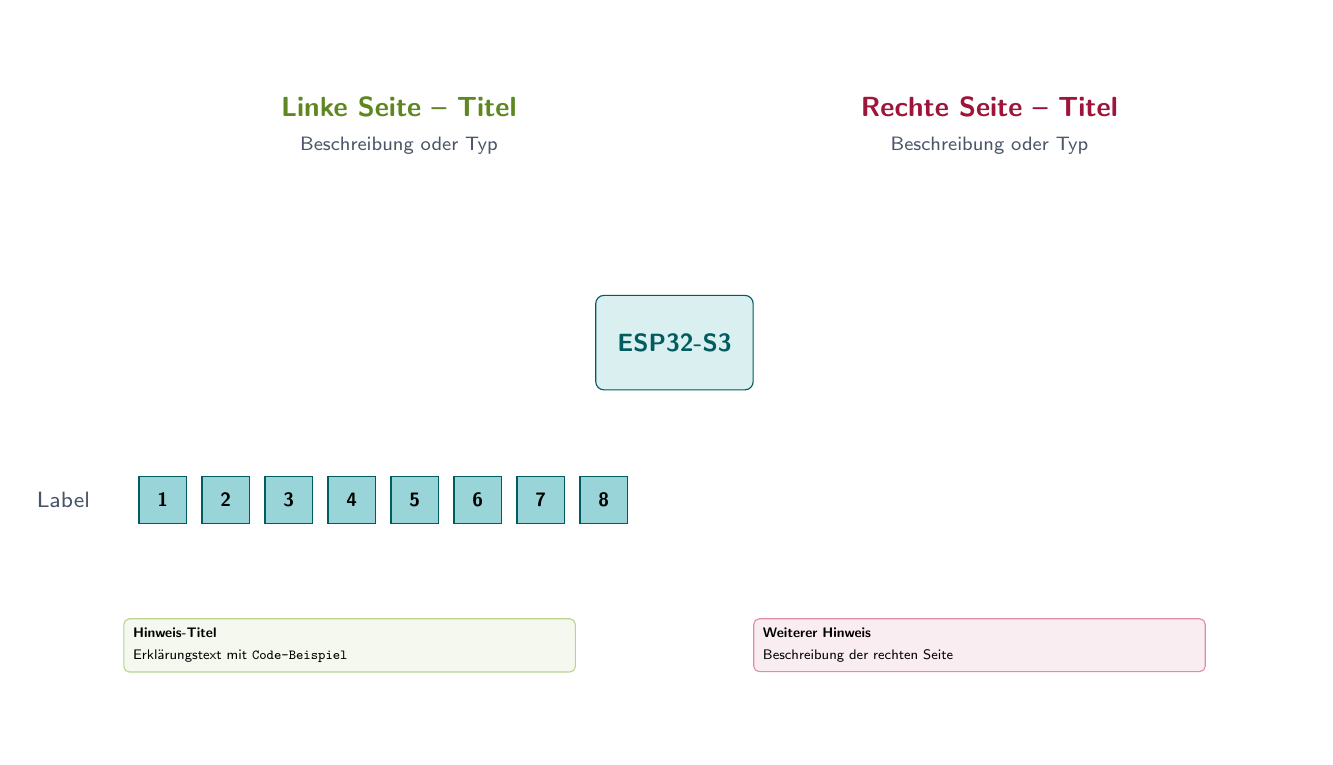
\begin{tikzpicture}[
  % === GRUNDSTILE ===
  % Box für Komponenten/Chips
  chip/.style={
    draw=ArduinoDark,
    fill=#1,
    minimum width=2cm,
    minimum height=1.2cm,
    rounded corners=3pt,
    font=\sffamily\bfseries\small
  },
  chip/.default=white,
  % Kleine Box für Bits/Werte
  bitbox/.style={
    draw=ArduinoDark,
    fill=#1,
    minimum width=0.6cm,
    minimum height=0.6cm,
    font=\sffamily\bfseries\scriptsize
  },
  bitbox/.default=ArduinoTeal!30,
  % Flip-Flop/Register-Box
  flipflop/.style={
    draw=ArduinoDark,
    fill=#1,
    minimum width=0.7cm,
    minimum height=0.7cm,
    font=\sffamily\bfseries\scriptsize
  },
  flipflop/.default=white,
  % Infobox
  infobox/.style={
    draw=#1!50,
    fill=#1!8,
    rounded corners=2pt,
    font=\sffamily\tiny,
    text width=5.5cm,
    align=left
  },
  infobox/.default=ArduinoTeal,
  % Labels
  lbl/.style={
    font=\sffamily\footnotesize,
    color=MutedText
  },
  bitlbl/.style={
    font=\ttfamily\tiny,
    color=MutedText
  },
  % Pfeile
  dataarrow/.style={
    draw=ArduinoTeal!70,
    line width=0.8pt,
    ->,
    >=Stealth
  },
  chainarrow/.style={
    draw=MutedText!60,
    line width=0.5pt,
    ->,
    >=Stealth
  }
]

% =============================================================================
% HINTERGRUND
% Anpassen: rectangle (xmin, ymin) -- (xmax, ymax)
% =============================================================================
\fill[white] (-1,-1) rectangle (15,8);

% =============================================================================
% TITEL (optional – auskommentieren wenn nicht benötigt)
% =============================================================================
% \node[font=\sffamily\bfseries\LARGE, color=ArduinoDark] 
%       at (7,7.5) {Haupttitel};
% \node[font=\sffamily\large, color=MutedText] 
%       at (7,6.9) {Untertitel oder Beschreibung};

% =============================================================================
% CONTENT – Hier den eigentlichen Inhalt einfügen
% =============================================================================

% --- Beispiel: Zwei-Spalten-Layout ---

% Linke Spalte – Überschrift
\node[font=\sffamily\bfseries, color=SuccessGreen!80!black] 
      at (3.5,7) {Linke Seite – Titel};
\node[font=\sffamily\scriptsize, color=MutedText] 
      at (3.5,6.5) {Beschreibung oder Typ};

% Rechte Spalte – Überschrift
\node[font=\sffamily\bfseries, color=RaspberryRed!80!black] 
      at (11,7) {Rechte Seite – Titel};
\node[font=\sffamily\scriptsize, color=MutedText] 
      at (11,6.5) {Beschreibung oder Typ};

% --- Beispiel: Chip/Komponente ---
\node[chip=ArduinoTeal!15, text=ArduinoDark] (esp) at (7,4) {ESP32-S3};

% --- Beispiel: Bit-Reihe ---
\node[lbl, anchor=east] at (-0.3,2) {Label};
\foreach \i/\val in {0/1, 1/2, 2/3, 3/4, 4/5, 5/6, 6/7, 7/8} {
  \node[bitbox=ArduinoTeal!40] at (\i*0.8+0.5,2) {\val};
}

% --- Beispiel: Infobox ---
\node[infobox=SuccessGreen, anchor=north west] at (0,0.5) {
  \textbf{Hinweis-Titel}\\[2pt]
  Erklärungstext mit \texttt{Code-Beispiel}
};

\node[infobox=RaspberryRed, anchor=north west] at (8,0.5) {
  \textbf{Weiterer Hinweis}\\[2pt]
  Beschreibung der rechten Seite
};

% =============================================================================
% BEISPIELE FÜR WEITERE ELEMENTE (auskommentiert)
% =============================================================================

% --- Verbindungspfeile ---
% \draw[dataarrow] (node1) -- (node2);
% \draw[dataarrow] (node1.east) -- ++(1,0) |- (node2.west);

% --- Schiebekette mit Pfeilen ---
% \foreach \i/\pin in {0/A, 1/B, 2/C, 3/D} {
%   \node[flipflop=SuccessGreen!25] (ff\i) at (\i*1,5) {\pin};
% }
% \foreach \i in {0,1,2} {
%   \pgfmathtruncatemacro{\j}{\i+1}
%   \draw[chainarrow] (ff\i.east) -- (ff\j.west);
% }

% --- Tabelle/Grid ---
% \foreach \x in {0,...,3} {
%   \foreach \y in {0,...,2} {
%     \node[bitbox=CodeBg] at (\x*0.8, \y*0.8) {};
%   }
% }

% --- Beschriftete Klammer ---
% \draw[decorate, decoration={brace, amplitude=5pt}] 
%       (0,3) -- (4,3) node[midway, above=5pt, font=\sffamily\tiny] {Beschriftung};

% --- Legende ---
% \node[font=\sffamily\scriptsize\bfseries, color=ArduinoDark, anchor=west] 
%       at (0,-0.5) {Legende:};
% \draw[dataarrow] (2,-0.5) -- ++(0.8,0) node[right, lbl] {Daten};
% \draw[RaspberryRed!70, line width=0.6pt, ->] (5,-0.5) -- ++(0.8,0) 
%       node[right, lbl] {Clock};

\end{tikzpicture}
\end{document}
